\section{Experiments} \label{sec: experiments}



\subsection{Experiment 1}
 Eliminating the need of cross-lingual information and we attempted to train NMT systems in a completely unsupervised manner, relying solely on monolingual corpora.


\subsubsection{Experimental architecture}
Architecture of the proposed system \ref{unsupervised_NMT}. For each sentence in language L1, the system is trained alternating two steps: denoising, which optimizes the probability of encoding a noised version of the sentence with the shared encoder and reconstructing it with the L1 decoder, and on-the-fly backtranslation, which translates the sentence in inference mode (encoding it with the shared encoder and decoding it with the L2 decoder) and then optimizes the probability of encoding this translated sentence with the shared encoder and recovering the original sentence with the L1 decoder. Training alternates between sentences in L1 and L2, with analogous steps for the latter.

 \begin{figure} [h]
    \center
    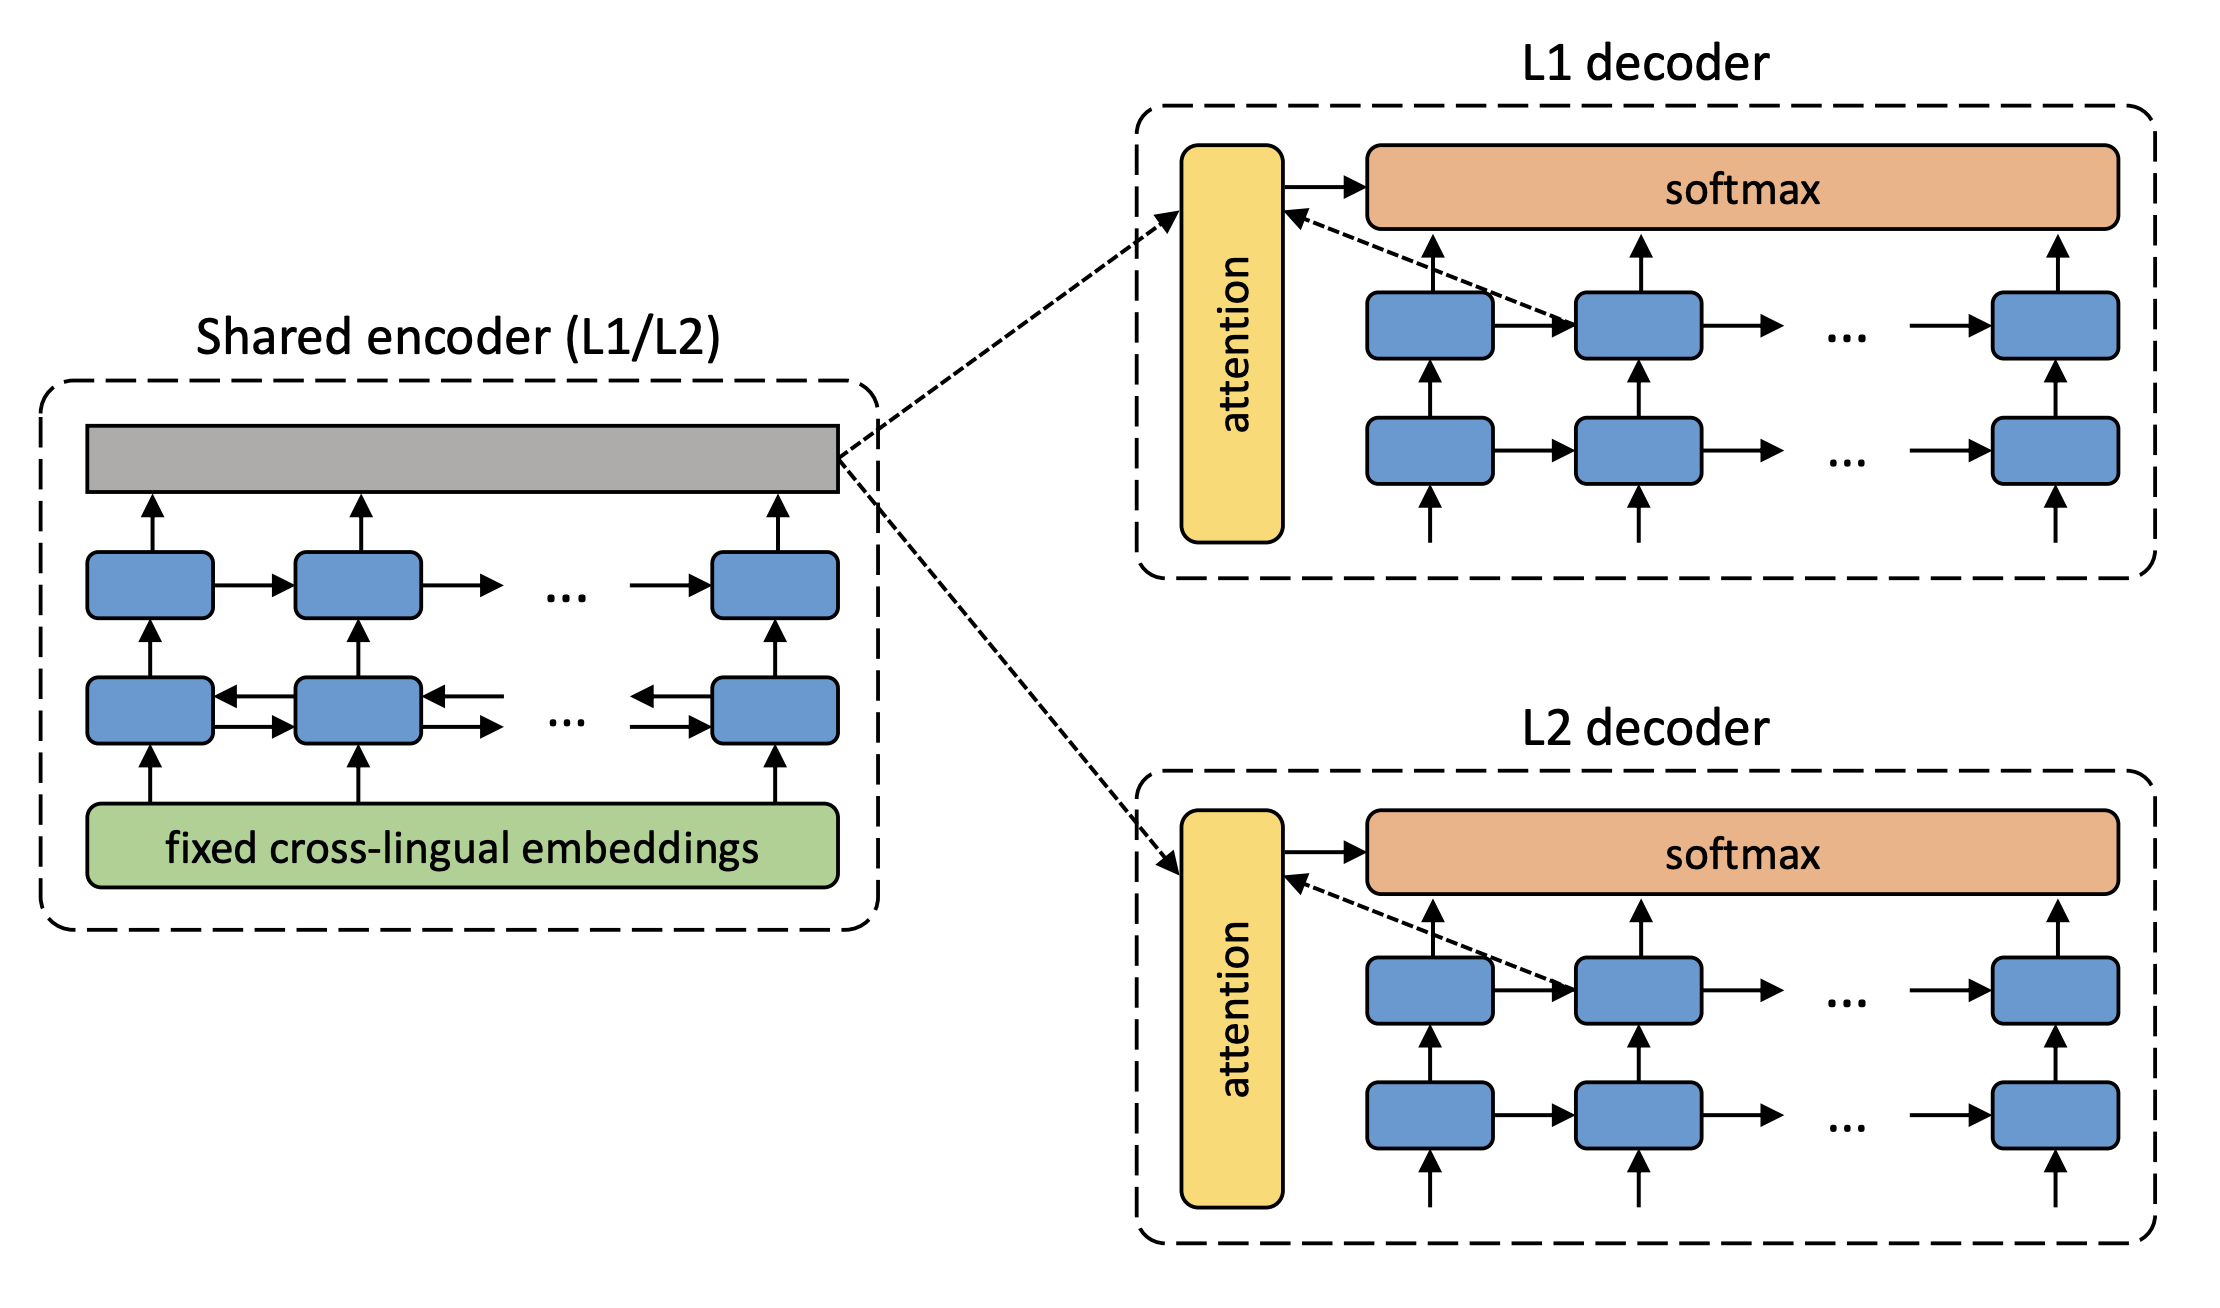
\includegraphics[width=8cm]{Figures/unsup_nmt.png}  
    \caption{Proposed System}
    \label{unsupervised_NMT}
\end{figure}

\subsubsection{Experimental settings}
\begin{enumerate}
    \item Unsupervised: This is the main scenario under consideration in our work, where the system has access to nothing but monolingual corpora.
    \item The systems are evaluated using tokenized BLEU scores as computed by the multi-bleu.perl script. 
    \item For the corpus preprocessing, tokenization and true casing using standard Moses are performed.
    \item Learning was done on the monolingual corpus of each language independently. 
    \item Experiments at the word level in this unsupervised scenario, limiting the vocabulary to the most frequent tokens and replacing the rest with a special token $<$UNK$>$. 
    \item Used the monolingual corpora to independently train the embeddings for each language using word2vec.
    \item we use the skip-gram model with ten negative samples, a context window of ten words, 300 dimensions, a sub-sampling of $10^{-5}$, and ten training iterations.
    \item The training of the proposed system itself is done using the procedure described with the cross-entropy loss function and a batch size of 50 sentences.
    

\end{enumerate}


\subsection{Experiment 2}
Experimental details about MASS pre-training and fine-tuning on a variety of language generation tasks are given as follows:


\subsubsection{Experimental architecture}

 \begin{figure} [h]
    \center
    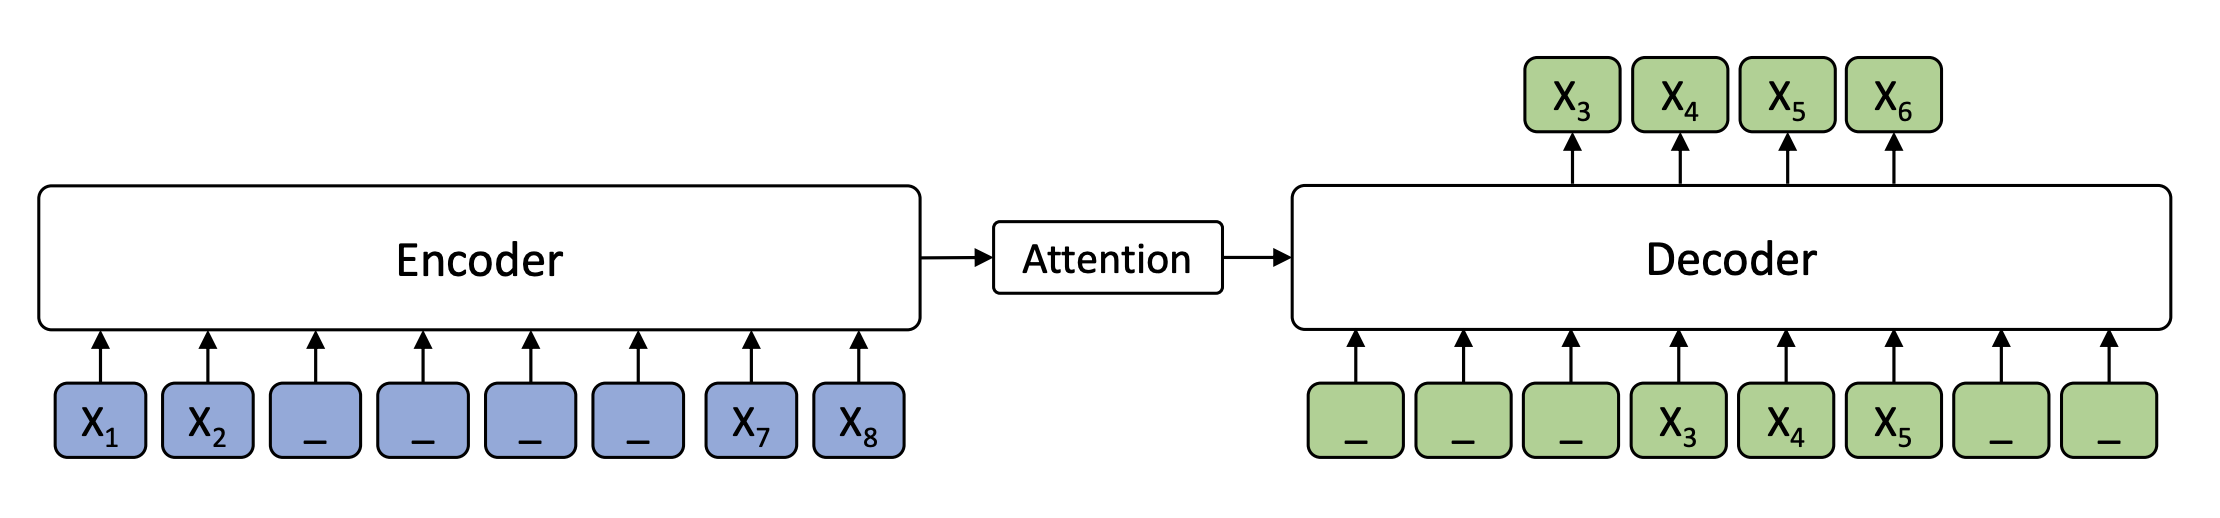
\includegraphics[width=8cm]{Figures/mass.png}  
    \caption{The Encoder-Decoder Framework}
    \label{en_dec_framework}
\end{figure}


\subsubsection{Experimental settings}
\begin{enumerate}
    \item Model Configuration : 
    Transformer as the basic model structure, which consists of 6-layer encoder and 6-layer decoder with 1024 embedding/hidden size and 4096 feed-forward filter size. 
    \item Pre-train the model on the monolingual data of the source and target languages.
    \item To distinguish between the source and target languages in neural machine translation task, a language embedding is added to each token of the input sentence for the encoder and decoder, which is also learnt end-to-end. 
    \item Dataset : 
\end{enumerate}